\section{Installing Vivado HL WebPACK}
Vivado HL WebPACK is a free program developed by Xilinx for creating designs and programming their
FPGAs, such as the one on the Nexys 4 and Basys 3 boards.

\subsection{Download}
First, create a free \href{https://www.xilinx.com/registration/create-account.html}
{Xilinx account}.
A verification email will be sent to the email provided.
Then, download Vivado 2018.2's
\href{https://www.xilinx.com/member/forms/download/xef.html?filename=Xilinx_Vivado_SDK_Web_2018.2_0614_1954_Win64.exe}
{web installer}.
This is a direct link to the Windows installer file, although you will have to sign in.
If you are on another OS or want to use the single-file download, the latest versions of Xilinx
software are available at \url{https://www.xilinx.com/support/download.html}.
During installation several gigabytes of files are downloaded so if you have a slow internet
connection it may be a good idea to install it at OU.

\subsection{Installation}
Run Xilinx\_Vivado\_SDK\_Web\_2018.2\_0614\_1954\_Win64.exe to start the installation.
On the welcome screen you can hit next, and then on the next screen type in your username and
password for the account you just created and hit next.

\begin{center}
    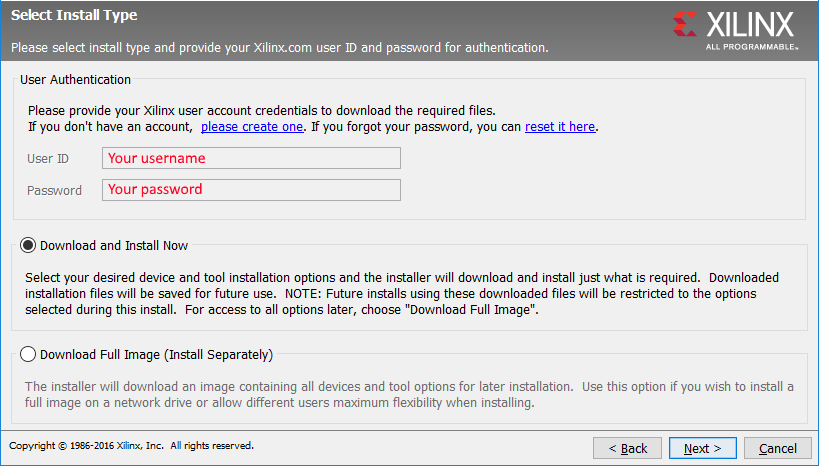
\includegraphics[width=\textwidth]{login_page}
\end{center}

On the next screen accept all the license agreements and hit next.
Then select Vivado HL WebPACK and hit next.

\begin{center}
    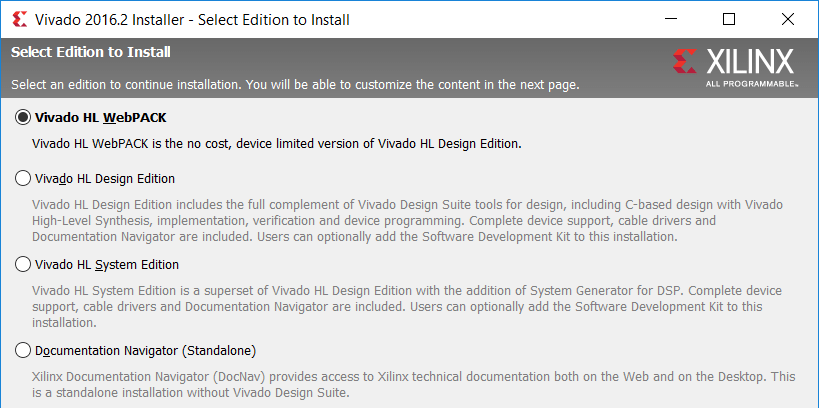
\includegraphics[width=\textwidth]{edition_page}
\end{center}

On the next screen you can select which parts of the software to install.
The defaults are fine, but if you’d like to save some space you can uncheck the SoC and UltraScale
sections, and the Kintex and Spartan under 7 series, as we won’t be using those devices.
Press next when you are done and on the next screen select where you would like to install Vivado.
Keep in mind that it will take over 10 GB of space on your hard drive.
Press next, review that everything is correct on this last screen, and then press install.
Enter your Xilinx account username and password again if a popup prompts you.

\begin{center}
    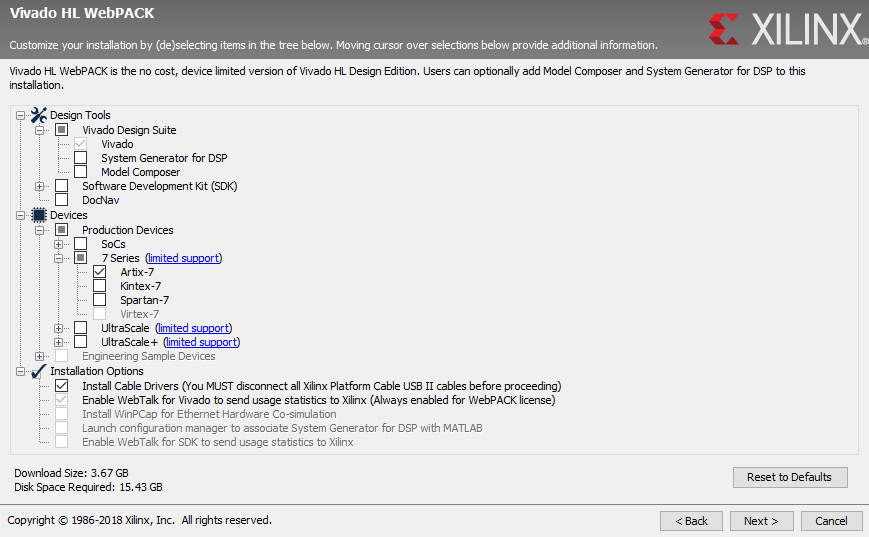
\includegraphics[width=\textwidth]{selection_page}
\end{center}

\begin{mdframed}[style=note]
    If after installing Vivado refuses to start and gives an error about the Microsoft Visual
    C++ 2012 Redistributable, try uninstalling all versions of the Microsoft Visual C++ 2012
    Redistributable, restart your computer, and try launching Vivado again.
    This seems to happen when a newer version than it expects is already installed on the system.
\end{mdframed}
